% Created by tikzDevice version 0.12.5 on 2024-01-20 17:25:12
% !TEX encoding = UTF-8 Unicode
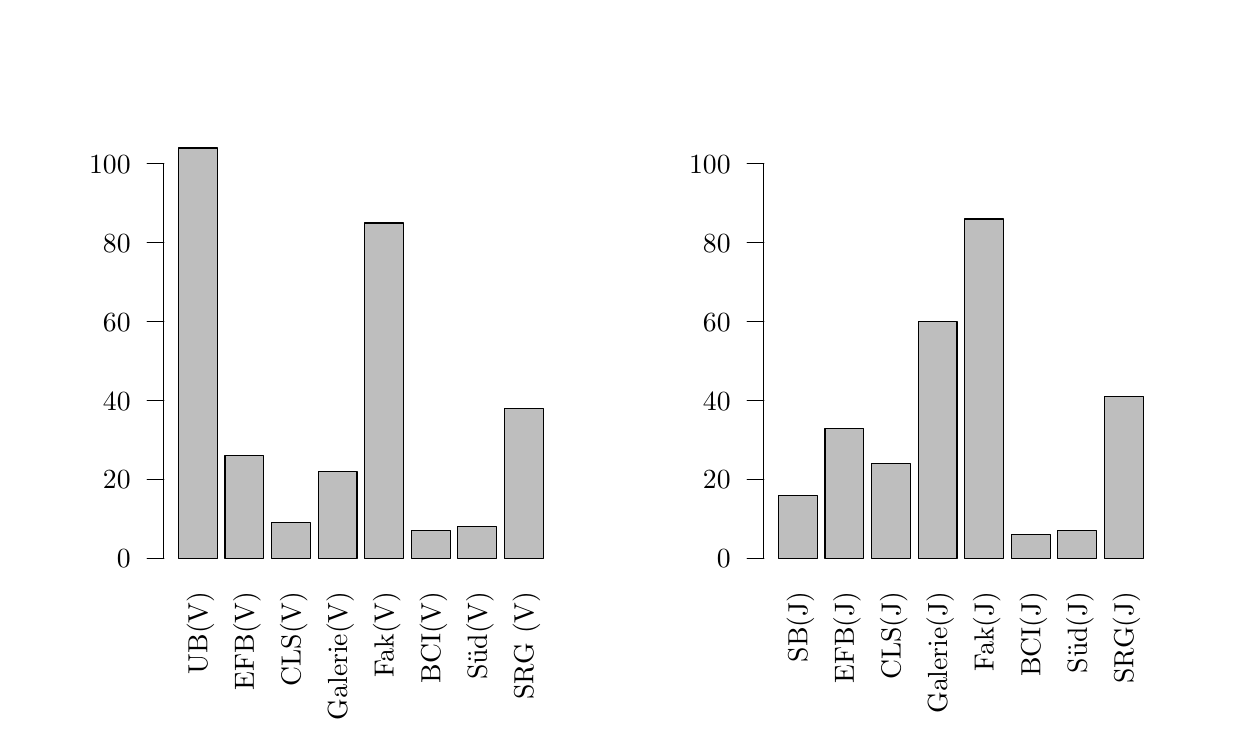
\begin{tikzpicture}[x=1pt,y=1pt]
\definecolor{fillColor}{RGB}{255,255,255}
\path[use as bounding box,fill=fillColor,fill opacity=0.00] (0,0) rectangle (433.62,252.94);
\begin{scope}
\path[clip] (  0.00,  0.00) rectangle (216.81,252.94);
\definecolor{drawColor}{RGB}{0,0,0}
\definecolor{fillColor}{RGB}{190,190,190}

\path[draw=drawColor,line width= 0.4pt,line join=round,line cap=round,fill=fillColor] ( 54.47, 61.20) rectangle ( 68.50,209.45);

\path[draw=drawColor,line width= 0.4pt,line join=round,line cap=round,fill=fillColor] ( 71.31, 61.20) rectangle ( 85.34, 98.26);

\path[draw=drawColor,line width= 0.4pt,line join=round,line cap=round,fill=fillColor] ( 88.14, 61.20) rectangle (102.17, 74.03);

\path[draw=drawColor,line width= 0.4pt,line join=round,line cap=round,fill=fillColor] (104.97, 61.20) rectangle (119.00, 92.56);

\path[draw=drawColor,line width= 0.4pt,line join=round,line cap=round,fill=fillColor] (121.81, 61.20) rectangle (135.84,182.36);

\path[draw=drawColor,line width= 0.4pt,line join=round,line cap=round,fill=fillColor] (138.64, 61.20) rectangle (152.67, 71.18);

\path[draw=drawColor,line width= 0.4pt,line join=round,line cap=round,fill=fillColor] (155.47, 61.20) rectangle (169.50, 72.60);

\path[draw=drawColor,line width= 0.4pt,line join=round,line cap=round,fill=fillColor] (172.31, 61.20) rectangle (186.34,115.37);
\end{scope}
\begin{scope}
\path[clip] (  0.00,  0.00) rectangle (433.62,252.94);
\definecolor{drawColor}{RGB}{0,0,0}

\node[text=drawColor,rotate= 90.00,anchor=base east,inner sep=0pt, outer sep=0pt, scale=  1.00] at ( 64.93, 49.20) {UB(V)};

\node[text=drawColor,rotate= 90.00,anchor=base east,inner sep=0pt, outer sep=0pt, scale=  1.00] at ( 81.77, 49.20) {EFB(V)};

\node[text=drawColor,rotate= 90.00,anchor=base east,inner sep=0pt, outer sep=0pt, scale=  1.00] at ( 98.60, 49.20) {CLS(V)};

\node[text=drawColor,rotate= 90.00,anchor=base east,inner sep=0pt, outer sep=0pt, scale=  1.00] at (115.43, 49.20) {Galerie(V)};

\node[text=drawColor,rotate= 90.00,anchor=base east,inner sep=0pt, outer sep=0pt, scale=  1.00] at (132.27, 49.20) {Fak(V)};

\node[text=drawColor,rotate= 90.00,anchor=base east,inner sep=0pt, outer sep=0pt, scale=  1.00] at (149.10, 49.20) {BCI(V)};

\node[text=drawColor,rotate= 90.00,anchor=base east,inner sep=0pt, outer sep=0pt, scale=  1.00] at (165.93, 49.20) {Süd(V)};

\node[text=drawColor,rotate= 90.00,anchor=base east,inner sep=0pt, outer sep=0pt, scale=  1.00] at (182.77, 49.20) {SRG (V)};

\path[draw=drawColor,line width= 0.4pt,line join=round,line cap=round] ( 49.20, 61.20) -- ( 49.20,203.75);

\path[draw=drawColor,line width= 0.4pt,line join=round,line cap=round] ( 49.20, 61.20) -- ( 43.20, 61.20);

\path[draw=drawColor,line width= 0.4pt,line join=round,line cap=round] ( 49.20, 89.71) -- ( 43.20, 89.71);

\path[draw=drawColor,line width= 0.4pt,line join=round,line cap=round] ( 49.20,118.22) -- ( 43.20,118.22);

\path[draw=drawColor,line width= 0.4pt,line join=round,line cap=round] ( 49.20,146.73) -- ( 43.20,146.73);

\path[draw=drawColor,line width= 0.4pt,line join=round,line cap=round] ( 49.20,175.24) -- ( 43.20,175.24);

\path[draw=drawColor,line width= 0.4pt,line join=round,line cap=round] ( 49.20,203.75) -- ( 43.20,203.75);

\node[text=drawColor,anchor=base east,inner sep=0pt, outer sep=0pt, scale=  1.00] at ( 37.20, 57.76) {0};

\node[text=drawColor,anchor=base east,inner sep=0pt, outer sep=0pt, scale=  1.00] at ( 37.20, 86.27) {20};

\node[text=drawColor,anchor=base east,inner sep=0pt, outer sep=0pt, scale=  1.00] at ( 37.20,114.77) {40};

\node[text=drawColor,anchor=base east,inner sep=0pt, outer sep=0pt, scale=  1.00] at ( 37.20,143.28) {60};

\node[text=drawColor,anchor=base east,inner sep=0pt, outer sep=0pt, scale=  1.00] at ( 37.20,171.79) {80};

\node[text=drawColor,anchor=base east,inner sep=0pt, outer sep=0pt, scale=  1.00] at ( 37.20,200.30) {100};
\end{scope}
\begin{scope}
\path[clip] (216.81,  0.00) rectangle (433.62,252.94);
\definecolor{drawColor}{RGB}{0,0,0}
\definecolor{fillColor}{RGB}{190,190,190}

\path[draw=drawColor,line width= 0.4pt,line join=round,line cap=round,fill=fillColor] (271.28, 61.20) rectangle (285.31, 84.01);

\path[draw=drawColor,line width= 0.4pt,line join=round,line cap=round,fill=fillColor] (288.12, 61.20) rectangle (302.15,108.24);

\path[draw=drawColor,line width= 0.4pt,line join=round,line cap=round,fill=fillColor] (304.95, 61.20) rectangle (318.98, 95.41);

\path[draw=drawColor,line width= 0.4pt,line join=round,line cap=round,fill=fillColor] (321.78, 61.20) rectangle (335.81,146.73);

\path[draw=drawColor,line width= 0.4pt,line join=round,line cap=round,fill=fillColor] (338.62, 61.20) rectangle (352.65,183.79);

\path[draw=drawColor,line width= 0.4pt,line join=round,line cap=round,fill=fillColor] (355.45, 61.20) rectangle (369.48, 69.75);

\path[draw=drawColor,line width= 0.4pt,line join=round,line cap=round,fill=fillColor] (372.28, 61.20) rectangle (386.31, 71.18);

\path[draw=drawColor,line width= 0.4pt,line join=round,line cap=round,fill=fillColor] (389.12, 61.20) rectangle (403.15,119.64);
\end{scope}
\begin{scope}
\path[clip] (  0.00,  0.00) rectangle (433.62,252.94);
\definecolor{drawColor}{RGB}{0,0,0}

\node[text=drawColor,rotate= 90.00,anchor=base east,inner sep=0pt, outer sep=0pt, scale=  1.00] at (281.74, 49.20) {SB(J)};

\node[text=drawColor,rotate= 90.00,anchor=base east,inner sep=0pt, outer sep=0pt, scale=  1.00] at (298.58, 49.20) {EFB(J)};

\node[text=drawColor,rotate= 90.00,anchor=base east,inner sep=0pt, outer sep=0pt, scale=  1.00] at (315.41, 49.20) {CLS(J)};

\node[text=drawColor,rotate= 90.00,anchor=base east,inner sep=0pt, outer sep=0pt, scale=  1.00] at (332.24, 49.20) {Galerie(J)};

\node[text=drawColor,rotate= 90.00,anchor=base east,inner sep=0pt, outer sep=0pt, scale=  1.00] at (349.08, 49.20) {Fak(J)};

\node[text=drawColor,rotate= 90.00,anchor=base east,inner sep=0pt, outer sep=0pt, scale=  1.00] at (365.91, 49.20) {BCI(J)};

\node[text=drawColor,rotate= 90.00,anchor=base east,inner sep=0pt, outer sep=0pt, scale=  1.00] at (382.74, 49.20) {Süd(J)};

\node[text=drawColor,rotate= 90.00,anchor=base east,inner sep=0pt, outer sep=0pt, scale=  1.00] at (399.58, 49.20) {SRG(J)};

\path[draw=drawColor,line width= 0.4pt,line join=round,line cap=round] (266.01, 61.20) -- (266.01,203.75);

\path[draw=drawColor,line width= 0.4pt,line join=round,line cap=round] (266.01, 61.20) -- (260.01, 61.20);

\path[draw=drawColor,line width= 0.4pt,line join=round,line cap=round] (266.01, 89.71) -- (260.01, 89.71);

\path[draw=drawColor,line width= 0.4pt,line join=round,line cap=round] (266.01,118.22) -- (260.01,118.22);

\path[draw=drawColor,line width= 0.4pt,line join=round,line cap=round] (266.01,146.73) -- (260.01,146.73);

\path[draw=drawColor,line width= 0.4pt,line join=round,line cap=round] (266.01,175.24) -- (260.01,175.24);

\path[draw=drawColor,line width= 0.4pt,line join=round,line cap=round] (266.01,203.75) -- (260.01,203.75);

\node[text=drawColor,anchor=base east,inner sep=0pt, outer sep=0pt, scale=  1.00] at (254.01, 57.76) {0};

\node[text=drawColor,anchor=base east,inner sep=0pt, outer sep=0pt, scale=  1.00] at (254.01, 86.27) {20};

\node[text=drawColor,anchor=base east,inner sep=0pt, outer sep=0pt, scale=  1.00] at (254.01,114.77) {40};

\node[text=drawColor,anchor=base east,inner sep=0pt, outer sep=0pt, scale=  1.00] at (254.01,143.28) {60};

\node[text=drawColor,anchor=base east,inner sep=0pt, outer sep=0pt, scale=  1.00] at (254.01,171.79) {80};

\node[text=drawColor,anchor=base east,inner sep=0pt, outer sep=0pt, scale=  1.00] at (254.01,200.30) {100};
\end{scope}
\end{tikzpicture}
